% Options for packages loaded elsewhere
\PassOptionsToPackage{unicode}{hyperref}
\PassOptionsToPackage{hyphens}{url}
%
\documentclass[
]{book}
\usepackage{amsmath,amssymb}
\usepackage{iftex}
\ifPDFTeX
  \usepackage[T1]{fontenc}
  \usepackage[utf8]{inputenc}
  \usepackage{textcomp} % provide euro and other symbols
\else % if luatex or xetex
  \usepackage{unicode-math} % this also loads fontspec
  \defaultfontfeatures{Scale=MatchLowercase}
  \defaultfontfeatures[\rmfamily]{Ligatures=TeX,Scale=1}
\fi
\usepackage{lmodern}
\ifPDFTeX\else
  % xetex/luatex font selection
\fi
% Use upquote if available, for straight quotes in verbatim environments
\IfFileExists{upquote.sty}{\usepackage{upquote}}{}
\IfFileExists{microtype.sty}{% use microtype if available
  \usepackage[]{microtype}
  \UseMicrotypeSet[protrusion]{basicmath} % disable protrusion for tt fonts
}{}
\makeatletter
\@ifundefined{KOMAClassName}{% if non-KOMA class
  \IfFileExists{parskip.sty}{%
    \usepackage{parskip}
  }{% else
    \setlength{\parindent}{0pt}
    \setlength{\parskip}{6pt plus 2pt minus 1pt}}
}{% if KOMA class
  \KOMAoptions{parskip=half}}
\makeatother
\usepackage{xcolor}
\usepackage{longtable,booktabs,array}
\usepackage{calc} % for calculating minipage widths
% Correct order of tables after \paragraph or \subparagraph
\usepackage{etoolbox}
\makeatletter
\patchcmd\longtable{\par}{\if@noskipsec\mbox{}\fi\par}{}{}
\makeatother
% Allow footnotes in longtable head/foot
\IfFileExists{footnotehyper.sty}{\usepackage{footnotehyper}}{\usepackage{footnote}}
\makesavenoteenv{longtable}
\usepackage{graphicx}
\makeatletter
\def\maxwidth{\ifdim\Gin@nat@width>\linewidth\linewidth\else\Gin@nat@width\fi}
\def\maxheight{\ifdim\Gin@nat@height>\textheight\textheight\else\Gin@nat@height\fi}
\makeatother
% Scale images if necessary, so that they will not overflow the page
% margins by default, and it is still possible to overwrite the defaults
% using explicit options in \includegraphics[width, height, ...]{}
\setkeys{Gin}{width=\maxwidth,height=\maxheight,keepaspectratio}
% Set default figure placement to htbp
\makeatletter
\def\fps@figure{htbp}
\makeatother
\setlength{\emergencystretch}{3em} % prevent overfull lines
\providecommand{\tightlist}{%
  \setlength{\itemsep}{0pt}\setlength{\parskip}{0pt}}
\setcounter{secnumdepth}{5}
% definitions for citeproc citations
\NewDocumentCommand\citeproctext{}{}
\NewDocumentCommand\citeproc{mm}{%
  \begingroup\def\citeproctext{#2}\cite{#1}\endgroup}
\makeatletter
 % allow citations to break across lines
 \let\@cite@ofmt\@firstofone
 % avoid brackets around text for \cite:
 \def\@biblabel#1{}
 \def\@cite#1#2{{#1\if@tempswa , #2\fi}}
\makeatother
\newlength{\cslhangindent}
\setlength{\cslhangindent}{1.5em}
\newlength{\csllabelwidth}
\setlength{\csllabelwidth}{3em}
\newenvironment{CSLReferences}[2] % #1 hanging-indent, #2 entry-spacing
 {\begin{list}{}{%
  \setlength{\itemindent}{0pt}
  \setlength{\leftmargin}{0pt}
  \setlength{\parsep}{0pt}
  % turn on hanging indent if param 1 is 1
  \ifodd #1
   \setlength{\leftmargin}{\cslhangindent}
   \setlength{\itemindent}{-1\cslhangindent}
  \fi
  % set entry spacing
  \setlength{\itemsep}{#2\baselineskip}}}
 {\end{list}}
\usepackage{calc}
\newcommand{\CSLBlock}[1]{\hfill\break\parbox[t]{\linewidth}{\strut\ignorespaces#1\strut}}
\newcommand{\CSLLeftMargin}[1]{\parbox[t]{\csllabelwidth}{\strut#1\strut}}
\newcommand{\CSLRightInline}[1]{\parbox[t]{\linewidth - \csllabelwidth}{\strut#1\strut}}
\newcommand{\CSLIndent}[1]{\hspace{\cslhangindent}#1}

% Load packages
\usepackage{booktabs}
\usepackage{amsthm}
\usepackage{svg}
\usepackage[english]{babel}
\usepackage{fancyhdr}

% Change "Chapter" to "Kapitel" throughout document
\addto\captionsenglish{\renewcommand{\chaptername}{Kapitel}}
% Change "Content" to "Indholdsfortegnelse"
\addto\captionsenglish{\renewcommand{\contentsname}{Indholdsfortegnelse}}


% Page layout
\makeatletter
\def\thm@space@setup{%
  \thm@preskip=8pt plus 2pt minus 4pt
  \thm@postskip=\thm@preskip
}
\makeatother
\usepackage{flafter}
\ifLuaTeX
  \usepackage{selnolig}  % disable illegal ligatures
\fi
\usepackage{bookmark}
\IfFileExists{xurl.sty}{\usepackage{xurl}}{} % add URL line breaks if available
\urlstyle{same}
\hypersetup{
  pdftitle={En befolkning blander sig},
  pdfauthor={Christian Albrekt Larsen og Hans-Peter Y. Qvist (Red.); Med bidrag fra Jeppe Fjeldgaard Larsen, Laciné E. Diop,\ldots{} Anders? Anna?},
  hidelinks,
  pdfcreator={LaTeX via pandoc}}

\title{En befolkning blander sig}
\author{Christian Albrekt Larsen og Hans-Peter Y. Qvist (Red.) \and Med bidrag fra Jeppe Fjeldgaard Larsen, Laciné E. Diop,\ldots{} Anders? Anna?}
\date{2024-05-29}

\begin{document}
\maketitle

{
\setcounter{tocdepth}{1}
\tableofcontents
}
\chapter*{Forord}\label{forord}
\addcontentsline{toc}{chapter}{Forord}

Måske et forord her.

I \hyperref[kap1]{kapitel 1} af \_\_\_\_\_, \ldots{}

I \hyperref[kap2]{kapitel 2} af \_\_\_\_\_, \ldots{}

I \hyperref[kap3]{kapitel 3, ``Grundskoler som mødested''}, af \href{https://vbn.aau.dk/da/persons/140717}{Jeppe Fjeldgaard Larsen}, \ldots{}

I \hyperref[kap4]{kapitel 4} af \_\_\_\_\_, \ldots{}

I \hyperref[kap5]{kapitel 5} af \_\_\_\_\_, \ldots{}

I \hyperref[kap6]{kapitel 6} af \_\_\_\_\_, \ldots{}

I \hyperref[kap7]{kapitel 7} af \_\_\_\_\_, \ldots{}

\chapter{En befolkning blander sig}\label{kap1}


\includegraphics[width=1\linewidth]{images/dalle-smeltedige}

\chapter{Partnerskabet og de blandede børn}\label{kap2}


\includegraphics[width=1\linewidth]{images/dalle-wedding}

\chapter{\texorpdfstring{Grundskoler som mødested (\textbf{WIP DO NOT CITE!})}{Grundskoler som mødested (WIP DO NOT CITE!)}}\label{kap3}

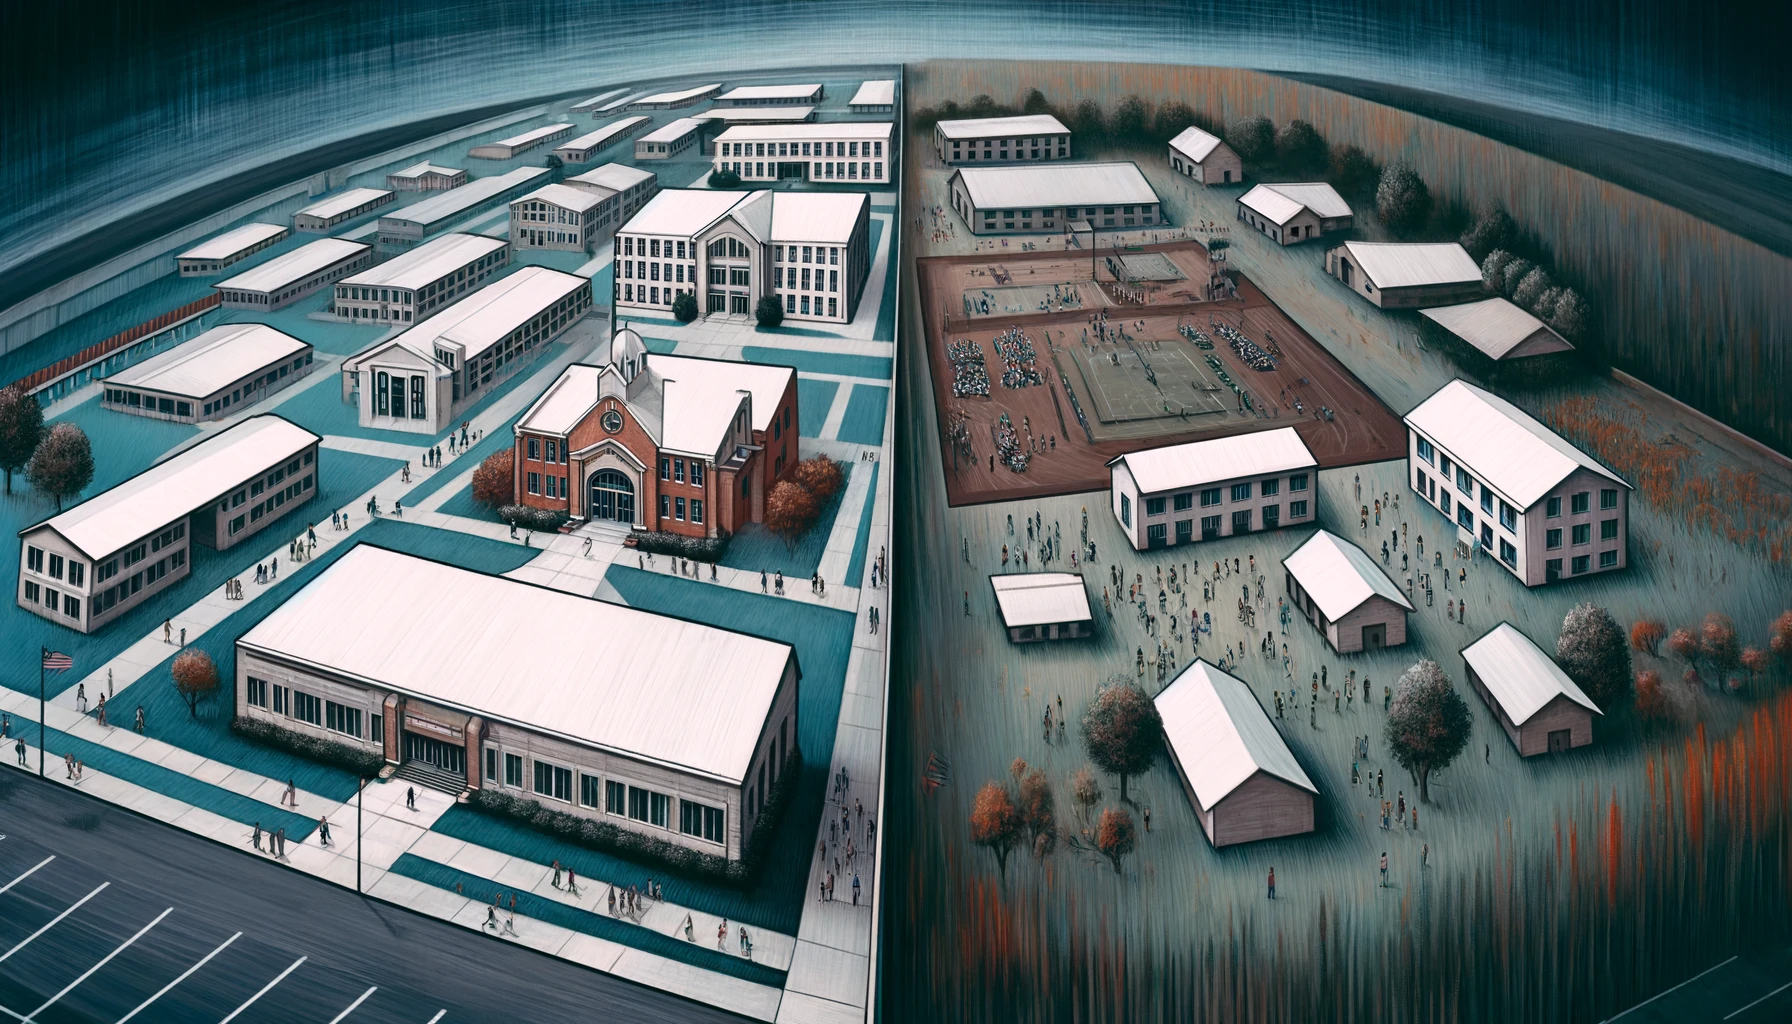
\includegraphics[width=1\linewidth]{images/dalle-schoolseg}

\section{Introduktion}\label{introduktion}

Jens Joel (MF, Socialdemokratiet) skriver i sin bog \emph{Fællesskaberen}, at ``tilliden, forståelsen og samhørigheden'' i Danmark er truet. Denne trussel mod den danske sammenhængskraft skyldes blandt andet, at vi ikke længere ``mødes {[}\ldots{]} i det, der før var `folkets skole'. I hvert fald ikke i tilstrækkelig grad'' (\citeproc{ref-joel2022}{Joel, 2002}, s. 11). Joel formår fortrinligt at tegne det grundlæggende solidariske og socialdemokratiske ideal for en fælles grundskole, hvor der er en tro på, at møder på tværs af forskellige baggrunde---hvad enten det er klasse eller etnisk tilhørsforhold---skaber tillid og tryghed i samfundet. I den socialdemokratiske forståelse af staten og samfundet er grundskolen dermed en helt fundamental ``byggesten i samfundet'' (Ibid., s. 11), fordi grundskolen er en institution, hvor børn kan interagere med hinanden, uanset deres ligheder med andre børn og deres forældre.

Men hvornår nåede (eller når) skolesegregeringen et niveau, hvor den ligefrem truer sammenhængskraften i vores samfund? Selvom noget forskning har forsøgt empirisk at definere den ''optimale sammensætning'' af børn i en klasse er ift. læring og sociale relationer (se nedenfor) eller ''tipping points'' for, hvornår etnisk danske familier fravælger den lokale skole på grund af en oplevelse af for stor andel minoriteter, er det i høj grad et politisk spørgsmål, hvornår segregering er ''for højt''. Faktum er imidlertid, at der er kommet flere ''minoritetsskoler'', hvor ingen---eller kun en mindre andel---børn med dansk oprindelse går i skole. Hvilket samtidigt betyder at der fortsat også er mange skoler, hvor ingen børn med indvandrerbaggrund går i skole. Det er sådanne ulige fordelinger af børn mellem skoler, vi forstår som skolesegregering. Selvom disse ''absolut segregerede'' skoler eksisterer, er skolesegregering typisk et spektrum af ulige fordeling af børn mellem skoler. Tag et stiliseret eksempel: I et område med tre skoler, hvor \(15\%\) af alle børn har indvandrerbaggrund. Én af skolerne har en andel af børn med indvandrerbaggrund på \(50\%\), mens de andre skoler har en andel på \(5\%\). Dette ville vi karakterisere som et segregeret område, da graden af eksponering mellem majoritets- og minoritetsgrupperne på skolerne ikke afspejler den eksponering, der ville være forventet givet befolkningssammensætningen. Konkret har Socialdemokratiet fremsat en ambition om, at ingen skoler skal have en andel af børn med \emph{ikke-vestlige} baggrunde over \(30\%\).

Selvom skæringspunktet på \(30\%\) tidligere er blevet fremhævet som et ``tipping point'' for, hvornår etnisk danske familier fravælger den lokale skole og igangsætter selvforstærkende segregeringsprocesser (\citeproc{ref-rangvid2010}{Rangvid, 2010}), vil jeg ikke tage stilling til eller give svar på, hvornår segregering er problematisk---og om det i alle situationer er ikke-ønskværdigt. I stedet vil jeg med dette kapitel empirisk beskrive grundtrækkene i omfanget af skolesegregering i den danske grundskole fra 1985 til 2020 som et bidrag og afsæt til videre debat.
Som jeg vil beskrive i det følgende, tenderer den store forfaldshistorie om et samfund, der ikke hænger sammen (i en kontekst af grundskolen), mod det overdrevne. Vi ser nemlig, at segregering generelt har været forholdsvis konstant og måske ikke så stærk som man kan få indtryk af i den offentlige debat. Men det er samtidigt også klart, at der er et stigende antal skoler, hvor børn med etnisk dansk baggrund udgør et numerisk mindretal, på trods af at børn med indvandrerbaggrund kun udgør \(12\%\) af alle børn i skolealderen i 2020, om end dette drejer sig om \(33\) skoler ud af \(1468\), hvor mere end halvdelen af eleverne har ''ikke-vestlige baggrunde''. Disse skoler er dog ikke tilfældigt fordelt, men placeret i bestemte kommuner og nabolag, der også er kendetegnet ved en relativt høj grad af boligsegregering. Med andre ord, selvom den store forfaldsfortælling måske ikke holder, er der stadig på lokale niveauer inden for kommuner i bestemte områder, hvor der kan være grund til bekymring og selvforstærkende segregeringsprocesser. En central pointe er, at den videre debat derfor må skelne mellem to dimensioner: Den store nationale skala, som måske kan bidrage til en meget generel fortælling om samfundstilstanden i Danmark, og den kommunale skala, hvor lokale og specifikke processer finder sted, men som ikke nødvendigvis kan generaliseres til at udtrykke en samfundsdiagnose.

Selvom skolesegregering på mange måder er et velbeskrevet fænomen i den internationale litteratur (se J. F. Larsen (\citeproc{ref-larsen2024a}{2024a}) for et overblik), er disse beskrivelser ofte grovkornede, da de er baseret på aggregerede tabeldata. Det betyder, at beskrivelserne er lavet på data, der er aggregeret på en høj geografisk eller administrativ skala, hvilket gør det umuligt at sige noget om relationen mellem de enkelte familiers sociale status eller hvilket skoledistrikt, de bor i, og graden af segregering. Med de danske registerdata er det muligt at lave en detaljeret og mere finkornet beskrivelse af fordelingen af børn mellem skoler, da disse data indeholder detaljeret information om hvert enkelt barn i alle skoler, inklusive privat- og friskoler, hvilket også sjældent er tilgængeligt i den internationale segregeringslitteratur. For eksempel kan vi detaljeret undersøge sammenhængen mellem bosætningsmønstre og tendenser i skoleindskrivninger. Med disse beskrivelser er det hensigten at nuancere og kvalificere de pågående debatter vedrørende den danske grundskole og dens rolle i de danske målsætninger for integration.

Kapitlet er opdelt i seks sektioner. Første sektion skitserer den danske kontekst og de centrale tematikker i skolesegregeringslitteraturen. Anden sektion præsenterer det danske skolelandskabs geografi og demografi. Tredje sektion måler graden af segregering på både nationalt og kommunalt niveau. Dette efterfølges af en præsentation og diskussion af, hvordan skolesegregering skal ses som et produkt af boligsegregering i sektion fire. Femte sektion beskriver og diskuterer, hvordan observerede grader af segregering skal tolkes i relation til faktiske møder mellem børn fra forskellige baggrunde. Sjette og sidste sektion konkluderer.

\section{NY OVERSKRIFT}\label{ny-overskrift}

I den internationale kontakt- og integrationslitteratur fremhæves skoler ofte som steder med potentiale til at nedbryde fordomme og stereotyper. Det vil sige, at kontakt i en skolekontekst på daglig basis kan være med til at skabe gensidig forståelse og konfrontere uberettigede fordomme og stereotyper mellem grupper, fordi børn får mulighed for at møde og se hinanden som individer fremfor som medlemmer af grupper. Dette potentiale for at nedbryde fordomme og stereotyper er dog ifølge teorien betinget af fire forhold, for at kontakt mellem grupper faktisk har en produktiv og positiv konsekvens : 1) Børnene befinder sig i en kontekst, hvor der er en autoritet (læreren), der strukturerer interaktioner og opgaver. 2) Børnene forventes at have et fælles mål (læring/eksamener). 3) De arbejder sammen om dette mål i overensstemmelse med skolens didaktiske principper. 4) Børnene har samme status i klassen (alle er elever underlagt læreren) (\citeproc{ref-allport1979}{Allport, 1979}; \citeproc{ref-pettigrew2006}{Pettigrew \& Tropp, 2006}; \citeproc{ref-tropp2005}{Tropp \& Pettigrew, 2005}). Det skal dog ikke underkendes, at der både er forskning og personlige historier, der beskriver tilfælde af diskrimination og fordomme mellem lærer og minoritetselever og elever imellem (\citeproc{ref-andersen2019}{S. C. Andersen \& Guul, 2019}). Lige status er derfor ikke nødvendigvis givet i en skolekontekst. Optimal kontakt i denne kontekst, som påpeget af Pettigrew (\citeproc{ref-pettigrew1998}{1998}), er ydermere betinget af, 5) at interaktionerne har venskabspotentiale. Da børn i en klasse har samme alder, og der som regel er en nogenlunde lige kønsfordeling i de fleste skoler, er der et principielt højt venskabspotentiale i de danske grundskoler (\citeproc{ref-mcpherson2001}{McPherson et al., 2001}).

International forskning har vist, at børn i såkaldte ``blandede skoler'', hvor elevsammensætningen ligner den egentlige befolkningssammensætning, har flere venskaber eller sociale relationer på tværs af etniske gruppeskel (\citeproc{ref-kruse2019}{Kruse \& Kroneberg, 2019}; \citeproc{ref-leszczensky2015}{Leszczensky \& Pink, 2015}). En anden forventet effekt er de såkaldte klassekammerateffekter (peer effects), som antager, at ressourcestærke elever kan være med til at hæve det faglige niveau for deres mindre ressourcestærke klassekammerater. Der pågår dog samtidigt diskussioner om, at både kontakt- og klassekammerateffekter i en metodologisk forstand er svære at isolere kausalt, da der forventeligt er grundlæggende problemer med selvselektion. For eksempel vil familier med de allerede laveste fordomme være mere tilbøjelige til at vælge den etnisk diverse distriktsskole (se f.eks. Hassan et al. (\citeproc{ref-hassan2022}{2022}) eller Hermansen \& Birkelund (\citeproc{ref-hermansen2015}{2015}) for en oversigt og diskussion).

\subsection{Den danske grundskole}\label{den-danske-grundskole}

Grundskolen i Danmark omfatter børn i alderen 6-16 år. Et særligt kendetegn ved den danske grundskole, sammenlignet med andre internationale skolesystemer, er fraværet af \emph{tracking}---også kaldet elevdifferentiering eller klasseopdeling---baseret på faglige evner. Det betyder, at børn ikke bliver placeret på bestemte skoler eller spor afhængigt af deres præstationer i de tidlige skoleår, som det er tilfældet i andre europæiske lande som Tyskland, Holland og England. I stedet fastlægger folkeskoleloven, at undervisningen i det danske skolesystem skal tilpasses det pågældende klasserum gennem undervisningsdifferentiering, målrettet klasserummet som det er fra børnehaveklassen frem til afgangseksamen i alle fag. Med det danske princip om undervisningsdifferentiering i stedet for elevdifferentiering er den danske grundskole dermed forventeligt et eksempel på optimal realisering af positive kontakt-effekter gennem sociale relationer på tværs af gruppetilhørsforhold i et barns formative år (\citeproc{ref-larsen2016}{C. A. Larsen, 2016}; \citeproc{ref-larsen2024c}{J. F. Larsen, 2024b}), når børnene tilbringer 10 år sammen i alle fag. Den aktuelle udfordring er imidlertid, at Danmark har en meget liberal og generøs skolevalgspolitik, hvor omkring 75\% af omkostningerne for hvert enkelt barn på en privatskole er statsfinansierede, mens den resterende fjerdedel er brugerbetaling. Dette gør privatskoler tilgængelige for en stor del af befolkningen---men samtidig utilgængelige for de laveste indkomstgrupper. Dette har skabt bekymringer for, at det socialdemokratiske princip om, at børn fra forskellige baggrunde går på samme skole, ikke længere bliver realiseret, fordi forældre frit kan vælge skoler til og fra.

Historisk set går retten til at bestemme over sit barns skolegang, under myndighedernes tilsyn, tilbage til Friskoleloven fra 1855. Selvom hver adresse er tilknyttet et skoledistrikt, hvor barnet har garanteret ret til indskrivning, tillader reglerne i dag, at familier frit kan søge om indskrivning på en anden folke-, privat- eller friskole, enten inden for kommunen eller i en anden kommune. Det eneste lovlige grundlag, en folkeskole kan afvise et barns optagelse på, er, hvis skolen ikke har plads, hvilket defineres som 28 børn i hver klasse i den pågældende årgang. Kommuner kan dog sænke den maksimale klassestørrelse til under 28 elever for at begrænse mulighederne for anvendelsen af skolevalg.

Til forskel kan fri- og privatskoler permanent bortvise børn eller afvise optagelse baseret på en individuel vurdering, hvilket folkeskoler også kunne før 2005. Grundet den decentrale finansiering af folkeskolen har de enkelte folkeskoler også store individuelle omkostninger ved at flytte et barn til et specialtilbud. I modsætning hertil har privatskolerne mindre udgifter i forbindelse med henvisninger til specialtilbud, idet de søger disse midler hos staten, hvor folkeskolerne skal finde midlerne i deres kommunalt allokerede budget.

Disse strukturelle forhold har affødt en grundlæggende bekymring for, at frit skolevalg og det private skolemarked vil føre til stigende ulighed og segregation mellem skoler på grund af socioøkonomiske forskelle i, hvem der i størst omfang vælger -- eller er i stand til -- at benytte sig af muligheden for frit skolevalg ved skolestart eller i løbet af barnets skolegang.

\subsection{Betingelser for møder i grundskolen}\label{betingelser-for-muxf8der-i-grundskolen}

Den primære hindring for realiseringen af kontakt- eller klassekammerateffekter i barndommen er først og fremmest omfanget af skolesegregering, da det konkret forhindrer kontakt mellem grupper af børn, hvis de ikke møder hinanden i deres daglige liv (\citeproc{ref-kruse2017}{Kruse, 2017}). Grundlæggende er segregering er et udtryk for en fysisk adskillelse af personer fra forskellige klassificerede grupper. Disse grupper kan være defineret ud fra majoritets-/minoritetsstatus, social status, køn og andre former for identitets-, økonomiske eller sociale faktorer. Typisk er segregering blevet diskuteret i forhold til (etnisk) boligsegregering, som angiver i hvilket omfang personer med indvandrerbaggrund bor i de samme boligområder som personer med dansk oprindelse---og omvendt. På samme måde udtrykker etnisk skolesegregering i hvilket omfang børn med dansk oprindelse kun (eller primært) går på skoler med andre børn med dansk oprindelse, og \emph{vice versa}. En vigtig pointe her er, at segregering refererer til fordelingen eller spredningen af de \emph{to} grupper, der sammenlignes. Det vil sige, at minoritetsgruppen ikke kan være segregeret uden at majoritetsgruppen også er det.

I Larsen (\citeproc{ref-larsen2024b}{2024c}, \citeproc{ref-larsen2024c}{2024b}) viser jeg, at det særligt er mekanismer på boligmarkedet, der driver skolesegregering, snarere end aktivt til- og fravalg af bestemte skoler, som ellers er den meget omtalte diagnose i den offentlige debat. For det første observerer vi, at børnefamilier gradvist bliver mere segregerede bosætningsmæssigt fra barnets fødsel indtil barnet begynder i børnehaveklassen. Dette indikerer, at familier, når eller hvis de flytter med børn i førskolealderen, er tilbøjelige til at bosætte sig i nabolag, hvor de andre beboere ligner dem selv. Samtidig ser vi, at når først barnet er startet i skole, er familier mindre tilbøjelige til at flytte, før barnet har afsluttet grundskolen (\citeproc{ref-larsen2024c}{J. F. Larsen, 2024b}). Disse bosætningsmønstre er centrale for at forstå skolesegregering i Danmark, da både nabolaget og skoledistriktet, som en familie bor---eller bosætter sig---i, hænger stærkt sammen med elevsammensætningen på den skole, som barnet går i (\citeproc{ref-larsen2024b}{2024c}). Dette forklares ved den simple observation, at mulighederne for at udnytte det frie skolevalg er betinget af de skoler, der er i nærheden af bopælen. Med andre ord betinger familiens bopæl deres reelle muligheder på skolemarkedet og er af større betydning end sociale gradienter i, hvilke familier der vælger privat- og friskoler (\citeproc{ref-bjerrenielsen2020}{Bjerre-Nielsen \& Gandil, 2020}; \citeproc{ref-larsen2024a}{J. F. Larsen, 2024a}). I et kausalitetsperspektiv betyder dette selvfølgelig, at vi ikke kan udelukke betydningen af skolevalget i en omvendt sammenhæng, idet valg af bolig også (in)direkte er et valg af skoledistrikt.

\section{Det danske skolelandskab}\label{det-danske-skolelandskab}

Når vi ser på det fysiske skolelandskab, det vil sige alle skoler og deres adresser, var det danske skolelandskab i 1985---det tidligste år, vi har data---bestående af 1327 skoler, hvoraf 246 var privat- eller friskoler. I 2020---det seneste år, vi har data for---var der samlet 1848 individuelle skoler, hvoraf 545 var privat- eller friskoler. Denne optælling ser bort fra alle specialtilbud, efterskoler og lignende og inkluderer kun institutioner, der i institutionsregistret er klassificeret som folkeskole eller privat- og friskole. I 2020 havde \(12\%\) af alle børn i niende klasse enten første eller anden generation indvandrerbaggrund. Til sammenligning var det kun under \(2\%\) i 1985.

Fra et geografisk perspektiv er der stor variation i, hvor tæt skoler ligger på hinanden. Dette har en indirekte betydning for omfanget af frit skolevalg, da områder med få skoler inden for relativt kort afstand også har færre reelle muligheder for at vælge alternative til distriktskolen, som diskuteret ovenfor. Figur \ref{fig:fig-3-1} visualiserer antallet af skoler inden for \(2 km\) fra det geografiske centrum af bopælssognet.

Kortet fungerer på sin vis som en indikator for befolkningstæthed, da der naturligvis vil være flere skoler i områder med mange familier. Men på grund af lave omkostninger ved etablering af private- eller friskoler vil nogle områder stadig have et relativt stort skolemarked, på trods af relativ lav befolkningstæthed. For at åbne en fri- eller privatskole er den eneste ikke-refunderbare direkte omkostning et gebyr på 20.000 kr. til ministeriet i forbindelse med anmeldelse om oprettelse af ny skole. Derfor gælder det, at familier i urbane områder generelt har flere skoler, de potentielt kan vælge mellem. De fleste husstande i Danmark har to skoler inden for en realistisk pendleafstand på \(2 km\), men som bemærkelsesværdige afvigelser fra gennemsnittet er der i København og Frederiksberg henholdsvis \(20\) og \(24\) skoler inden for \(2 km\).

\begin{figure}
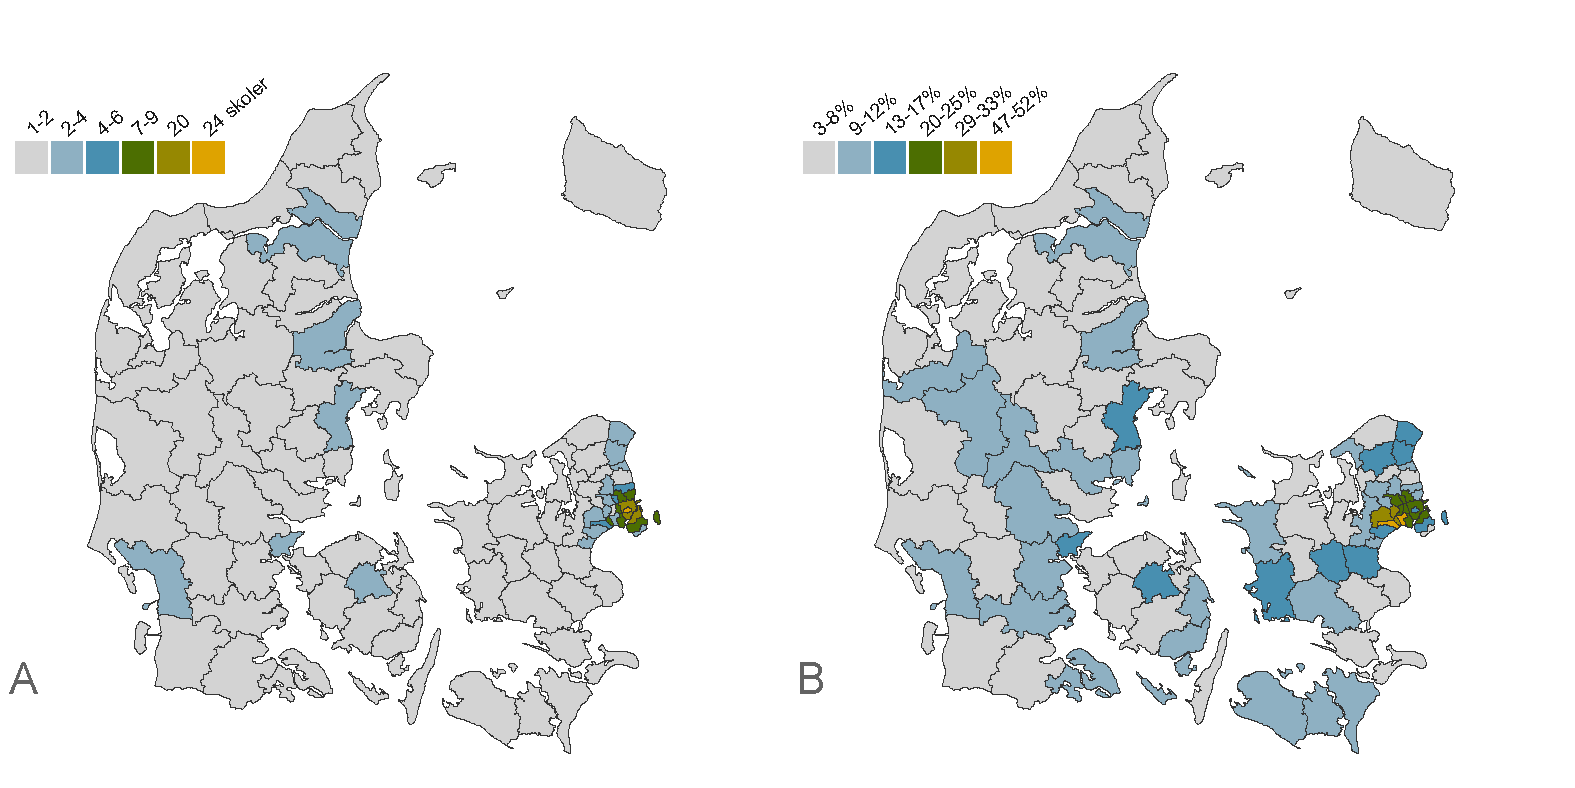
\includegraphics[width=1\linewidth]{images/figur_3_1c_distance_antal} \caption{Gennemsnitligt antal skoler inden for 2 km af bopælsadressen (A) og koncentration af børn med ikke-vestlig indvandrerbaggrund i skolealderen i 2020 (B) (B). <br> <br> Note: * Afstandene til skolen er baseret på den euclidiske afstand fra bopælssognets centroid til de geografiske koordinater for skolens adresse. Ikke-vestlig indvandrerbaggrund inkluderer børn, hvor begge eller én af forældrene er første generations immigrant fra et ikke-vestligt land.*}\label{fig:fig-3-1}
\end{figure}

Det centrale her er, at fordi børnefamilier med indvandrerbaggrund er koncentreret i urbane områder (se \hyperref[kap1]{kapitel 1}), er konsekvensen en stærk korrelation mellem store skolemarkeder (områder med mange skoler at vælge mellem) og områder med høj etnisk diversitet. Figuren giver dermed et deskriptivt indblik i, hvordan det fysiske skolelandskab og demografiske forhold kan spille sammen. I urbane områder, såsom hovedstadsområdet, er der en høj koncentration af skoler, hvilket giver mange muligheder for skolevalg. Samtidig er der også en højere koncentration af børn med indvandrerbaggrunde, særligt fra ikke-vestlige baggrunde. Dette skaber et potentiale for både høj etnisk diversitet i skolerne og for etnisk skolesegregering, da familier har mulighed for at vælge skoler væk fra dem med høj andel af elever med ikke-vestlig baggrund. I forstæderne og mindre byer er der færre skoler, hvilket betyder flere strukturelle begrænsninger for skolevalg. Samtidig er koncentrationen af familier med indvandrerbaggrund tilsvarende lavere. I kontrast er der i landdistrikterne få skoler inden for pendleafstand fra bopælen og dermed begrænsede muligheder for skolevalg. Her er koncentrationen af familier med ikke-vestlige baggrunde meget lav, hvilket forventeligt leder til lav diversitet på skolerne og en høj grad af strukturelt betinget skolesegregering grundet en lille minoritetsgruppe. Sammenfattende illustrerer figuren hvordan forholdet mellem strukturelle betingelser givet ved det fysiske skolelandskab og demografiske forhold mellem forskellige geografiske områder kan påvirke mulighederne for skolevalg og niveauet af etnisk diversitet i skolerne, og understreger de strukturelle forhold, der kan føre til skolesegregering.

Med andre ord, i urbane områder er der på den ene side et strukturelt potentiale for ``blandede'' skoler med høj gensidig eksponering mellem majoritets- og minoritetsgrupper, fordi der er en relativ høj koncentration af familier med indvandrerbaggrunde. Det vil sige, at de fleste familier med dansk oprindelse har en stor sandsynlighed for at møde andre familier, der ikke ligner dem selv. Samtidig er der dog også et stort strukturelt potentiale for etnisk skolesegregering, der overstiger det niveau, som er betinget af etnisk boligsegregering. Dette skyldes, at der er nok skoler til, at familier realistisk kan undgå de mindre attraktive skoler ved at indskrive deres børn på andre skoler (\citeproc{ref-larsen2024b}{J. F. Larsen, 2024c}). Disse mindre attraktive skoler er---rimeligt eller ej---ofte associeret med en høj andel elever fra ikke-vestlige immigrantbaggrunde. De fleste familier angiver, når de bliver spurgt, at det vigtigste kriterium i skolevalget er barnets trivsel og skolens ``faglige kvalitet'' (\citeproc{ref-epinion2017}{Epinion, 2017}). Denne kvalitet kan dog ofte være svær at vurdere i praksis, så det udefra observerbare elevgrundlag bliver ofte en målestok for vurderet kvalitet og skolens omdømme (\citeproc{ref-rambuxf8ll2011}{Rambøll, 2011}). Empiriske studier viser, at familier med de højeste uddannelser også er mest sensitive over for antallet af ``ikke-indfødte'' elever på en skole (\citeproc{ref-bjerrenielsen2020}{Bjerre-Nielsen \& Gandil, 2020}; \citeproc{ref-karsten2003}{Karsten et al., 2003}; \citeproc{ref-nielsen2019}{Nielsen \& Andersen, 2019}). Efter trivsel og ``faglig kvalitet'' er ``afstand til skolen'' fra bopælen også et vigtigt kriterium for mange forældre (\citeproc{ref-epinion2017}{Epinion, 2017}). Derfor kan sammenhængen mellem antallet af skoler og koncentrationen af børn med ikke-vestlig indvandrerbaggrund være med til at forstå de udfordringer og muligheder, der eksisterer for integration og skolevalg i forskellige geografiske områder. Urbane områder med mange skoler og høj diversitet står over for udfordringen med at sikre, at kontakt- og klassekammerateffekter kan realiseres på grund af segregeringsprocesser, mens landdistrikter kan være udfordret af begrænsede skolevalgmuligheder.

\section{Segregering i det danske skolelandskab}\label{segregering-i-det-danske-skolelandskab}

Når vi måler graden af segregering, er det mest anvendte mål for (skole)segregering \emph{Dissimilarity} (\(D\)) indekset, men også \emph{Separation} (\(S\)) indekset har en vis udbredelse . Begge mål kan have værdierne 0-1, og i empiriske cases vil de to mål essentielt altid være korrelerede. \(S\) er typisk noget lavere end \(D\), da \(S\) korrigerer for størrelsen af skoler og grupper, mens \(D\) ikke gør (se \hyperref[bilag1]{bilag A} for yderligere information). Den grundlæggende forskel mellem de to mål er, at \(D\) måler graden af ulige fordeling, mens \(S\) måler graden af polarisering.

Lidt simplificeret vil det sige, at \(D\) måler, hvor mange fra én af grupperne i sammenligningen, der hypotetisk skal flyttes til en ny skole for, at fordelingen er ``lige''. ``Lige fordeling'' er i denne kontekst et udtryk for en situation, hvor samtlige skoler i en kommune/nation har samme andel minoriteter som på kommunalt/nationalt niveau. Det vil sige, at indekset måler i hvilket omfang andelene på de enkelte skoler ligner den overordnede befolkningssammensætning i området. Et lavt \(D\)-indeks udtrykker altså, at alle eller de fleste skoler har en andel af hver gruppe, der spejler størrelserne af grupperne i populationen. Modsat udtrykker et højt \(D\)-indeks, at få skoler optager næsten alle minoriteter og vice versa. For eksempel, i et område med tre skoler og en population, hvor \(15\%\) har indvandrerbaggrund, skal alle skoler have en andel på \(15\%\) for ingen segregering, hvilket svarer til \(D=0\). Indekset skelner dog ikke til de absolutte tal, så om \(15\%\) udgøres af \(15\) ud af \(100\) elever eller \(150\) ud af \(1000\) gør ingen forskel i indekset. I en substantiel og levet kontekst er det selvfølgelig af betydning.

Med det samme eksempel for den hypotetiske kontekst er størrelsen af skolerne af betydning for målet for \(S\), idet det udtrykker hvilket omfang børn fra forskellige baggrunde er isoleret fra hinanden. Hvis én skole har en andel elever med indvandererbaggrund på \(15\%\) og de andre to har \(5\%\) og alle skoler har en størrelse på 25 elever, vil \(S \approx 0,05\). Hvis elevtallet var \(100\) på skolen med en andel på \(15\%\) og fortsat 25 på de to andre skoler ville \(S \approx 0,025\), da flere børn fra den samlede majoritetsgruppen vil være eksponeret til børn med indvandrerbaggrund. \(S\) er derfor en kvantifisering af den gennemsnitlige eksponering til ens egen gruppe (eller isolering fra sin udgruppe), kontrolleret for den relative størrelse af grupperne, da en lille minoritetsgruppe kan være isoleret som en ren tilfældighed, mens en relativ stor minoritetsgruppe som er isoleret, vil som udgangspunkt være et udtryk for en systematisk sortering og ikke en tilfældighed. Med andre ord, hvor stor en andel børn med dansk oprindelse går det gennemsnitlige barn med dansk oprindelse i skole med---og omvendt for børn med indvandrerbaggrund. Det er derfor grundlæggende et mål for gennemsnitlig eksponering til sin egen gruppe mod eksponering til en anden gruppe. \(S=0\) udtrykker en fordeling mellem skoler, hvor børn på alle skoler har den samme grad af intergruppe eksponering. Derfor, og igen en smule simplifiseret skal \(S\), tolkes som omfanget af eksponering mellem to grupper og kan dermed også tolkes som et spektrum af polarisering mellem to grupper.

\subsection{National skala}\label{national-skala}

På landsplan måles segregeringen til \(D = 0,44\) og \(S = 0,16\) i 2020, se Figur \ref{fig:fig-3-2}. Som diskuteret indledningsvis, præcis hvornår segregering er ``for høj'' er delvist et politisk og normativt spørgsmål. Dog peger den klassiske (amerikanske) segregeringslitteratur på, at \(D<0,3\) anses som lavt, mens \(D>0,6\) betragtes som højt (\citeproc{ref-massey1994}{Massey \& Denton, 1994}). I en segregeringskontekst vil \(S=0,6\) betragtes som meget højt, da der vil være en betydelig mængde skoler, der (næsten) udelukkende består af enten majoritets- eller minoritetsbaggrund, og den gennemsnitlige eksponering til ens egen gruppe er markant større end den ville være under forudsætning af tilfældige fordelinger mellem skoler. Nedenfor i Figur \ref{fig:fig-3-2} ses udviklingen af begge mål for segregering. Grundlæggende har graden af skolesegregering på begge dimensioner været nogenlunde stabil siden starten af 00'erne. Bemærk, at som det er diskuteret ovenfor, er to grundlæggende forskellige dimensioner af fordeling af børn, der måles. Vi ser derfor, at de to mål for segregering tilsyneladende konvergerer frem mod 00'erne. Dette skyldes ændrede strukturelle forhold. Simpelt sagt, i 1985 var der for få børn med indvandrerbaggrund og for mange skoler til, at disse børn kunne have været ``ligeligt'' fordelt i henhold til \(D\)-indekset. En vis grad af skolesegregering har derfor været en strukturel betingelse. Til gengæld viser \(S\)-indekset, at denne gruppe af børn med indvandrerbaggrund i meget stort omfang har gået på skoler, hvor de har udgjort en numerisk minoritet. Igen en strukturel betingelse, når minoritetsgruppen udgør en lille gruppe i numerisk forstand. Gruppen har ikke været stor nok til, at den i praksis kunne have udgjort en numerisk majoritet på enkelte skoler. I takt med at gruppen af børn med indvandrerbaggrund bliver større relativt til gruppen af børn med dansk oprindelse, er der altså de nødvendige strukturelle betingelser for, at flere---hvis ikke de fleste---skoler kan optage børn med indvandrerbaggrund. Dette bliver til en vis grad realiseret. Men, som vi ser med et parallelt stigende \(S\)-indeks, kommer der fortsat flere skoler, hvor børn med indvandrerbaggrund udgør en relativt stor andel eller den numeriske majoritet på skolen. Dette har en klar strukturel tolkning. Indvandrerfamilier bosætter sig disproportionelt i hovedstadsområdet og de største kommuner (se se \hyperref[kap1]{kapitel 1}), hvilket muliggør eksistensen af skoler, hvor størstedelen udgøres af børn med indvandrerbaggrund. Konvergeringen, hvor det ene mål falder og det andet stiger, tolkes derfor som primært at være drevet af ændrede strukturelle betingelser for segregering---herunder historiske bosætningsmønstre blandt familier med indvandrerbaggrund.

\begin{figure}
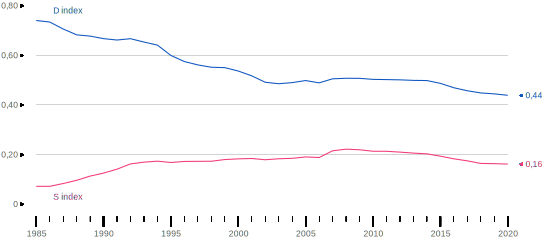
\includegraphics[width=1\linewidth]{images/figur_3_2} \caption{Etnisk skolesegregering i Danmark}\label{fig:fig-3-2}
\end{figure}

Graden af segregering i Danmark vil derfor være at betragte som moderat i dag, hvilket kan være overraskende for nogle, givet den aktuelle offentlige debat, hvor man kunne tro, at den har været voldsomt stigende. På nationalt plan har segregeringen faktisk været faldende. Selvom fordelingen har været skæv, især frem til årtusindskiftet, har der ikke været egentlig polarisering, hvor minoritetsgrupper har gået på skoler med meget begrænset kontakt til majoritetsgrupper. Med andre ord, graden af segregering (\(D\)) har tidligere grundlæggende været strukturelt betinget, idet der ikke har været tilstrækkeligt mange minoritetsbørn, og de har været koncentreret i for få kommuner til, at de praktisk kunne fordeles blandt alle skoler i Danmark. Fordelingen af denne gruppe børn ville altså være skæv, selv ved en tilfældig fordeling af børn mellem skolerne. Samtidig har vi dog set en stigning i \(S\)-indekset frem til omkring 2007. Denne stigning skal særligt ses i lyset af bosættelsesmønstrene blandt immigranter. Når visse kommuner oplever en relativ koncentration af immigranter, vil der i numerisk forstand være ``nok'' børn med indvandrerbaggrund til at udgøre en større andel af elevgrundlaget på en skole. Især fremkomsten af muslimske friskoler bidrager til polarisering i en segregeringskontekst, især når der samtidig også er skoler, hvor alle børn har dansk oprindelse. I en substantiel tolkning kan denne grad af segregering oversættes til faktisk intergruppe eksponering. Det vil sige, for det \emph{gennemsnitlige} barn med indvandererbaggrund, hvor stor en andel af den potentielle sociale gruppe på en grundskole har indvanderernaggrund, og \emph{vice versa}? I 1985, har det gennemsnitlige barn med indvandererbaggrund en \emph{potentiel} eksponering til børn andre børn med indvandererbaggrunde på deres skole på \(16\%\). I 2020, er denne \emph{potentielle} eksponering steget til \(35\%\). For det gennemsnitlige barn med dansk oprindelse, var eksponeringen til børn med indvandererbaggrunde \(7\%\) i 1985 og \(19\%\) i 2020.

\subsection{Lokal skala}\label{lokal-skala}

Når segregering måles på en stor skala, som f.eks. på landsplan, skjules betydelige lokale variationer i gennemsnittet. I Figur \ref{fig:fig-3-3} er begge mål for segregering og deres korrelation illustreret. Figuren skal læses således, at segregering kan være lav/høj målt som \(D\) (rødlige farver: horizontale kvadranter) eller lav/høj målt som \(S\) (blålige farver: vertikale kvadranter). Idet de to mål ofte korrelerer i praksis, ser vi også, at de to mål for segregering ofte er lav/lav eller høj/høj på begge dimensioner (lilla farver: diagonale kvadranter fra nedre-venstre til øvre-højre). Disse lokale variationer viser, at selvom landsplan-data kan indikere en moderat segregering, kan der være betydelige forskelle mellem kommuner. Nogle kommuner kan have høj polarisering uden en ulige fordeling af elever på skolerne, mens andre kan have en ulige fordeling uden stærk polarisering. Dette illustrerer vigtigheden af at analysere segregering på forskellige geografiske niveauer for at få et mere nuanceret billede af situationen.

Ved at måle skolesegregering i de enkelte kommuner over tid, med fokus på år 1985 og 2020, ser vi i 1985, at segregeringsniveauet lå mellem \(D=0,2-0,4\) i nogle kommuner, mens det i andre kommuner var over \(D>0,4\). Det er dog væsentligt at bemærke, at ingen af disse kommuner havde høj segregering, hvis det måles som polarisering (\(S\)). Alle kommuner havde et segregeringsniveau under \(0,1\) målt som \(S\) i 1985. Tolkningen af disse to dimensioner af segregering i sammenhæng er derfor, at selvom der isoleret set var relativt høje grader af segregering i flere kommuner i 1985, skyldtes dette i høj grad strukturelle forhold, som diskuteret ovenfor. Med andre ord, selvom \(D\)-indekset viste en ulige fordeling af elever med indvandrerbaggrund, viste \(S\)-indekset, at der ikke var en høj grad af polarisering, hvilket betyder, at eleverne stadig havde en vis grad af kontakt på tværs af grupper.

Dette ændrer sig dog frem mod 2020, hvor vi ser, at mange kommuner har både en høj grad af ulige fordeling af minoritetsbørn mellem skoler (\(D\)) og at børn med indvandrerbaggrund udgør en betydelig del af elevgrundlaget på bestemte skoler (\(S\)) og vice versa for børn med dansk oprindelse. Med andre ord, segregering målt som henholdsvis \(D\) og \(S\) begynder at korrelere stærkere over tid, hvilket betyder, at skolesegregeringen i mange kommuner i dag er præget af ikke bare ulige fordeling mellem skoler som en strukturel betingelse, men også polarisering mellem skoler. Dette indebærer, at der er stadig flere skoler, hvor børn med indvandrerbaggrund udgør en større del af elevgrundlaget, samtidigt med at andre skoler stort set ingen elever med indvandrerbaggrund har. Denne udvikling kan tilskrives de ændrede bosætningsmønstre og det frie skolevalg, som giver familier mulighed for at vælge skoler, der i højere grad matcher deres egne præferencer og socioøkonomiske baggrund. Dette skaber et komplekst billede, hvor både strukturelle og valgfrie faktorer bidrager til den nuværende segregeringsdynamik i danske skoler. I relation til konsekvenserne af fritskole valg skyldes udviklingen også delvist det private skolemarked, hvor for eksempel de muslimske friskoler i høj grad bidrager til kommunal skolesegregering. Disse skoler har både en ren minoritetskoncentration og er dermed polariserede i forhold til de andre lokale skoler med få eller ingen minoritetsbørn. Derudover bidrager sådanne skoler til, at minoritetsbørn ``trækkes ud'' af omkringliggende lokale skoler, hvilket øger koncentrationen af børn med dansk oprindelse på disse skoler, hvilket igen øger polariseringen yderligere mellem lokale skoler. Den samme proces gør sig selvfølgelig gældende for alle privat- og friskoler, der henvender sig til bestemte grupper, såsom kristne eller jødiske skoler. Disse skoler tiltrækker bestemte befolkningsgrupper, hvilket medfører en yderligere segregering og polarisering i de kommunale skoler. Derfor kan vi tolke det således, at selvom den overordnede segregering er moderat og faldende, er der stadig lokalt betingede udfordringer med polarisering, især i områder med høj koncentration af indvandrere. Dette skaber et komplekst billede, hvor nationale tendenser ikke nødvendigvis afspejler de lokale realiteter, og hvor både strukturelle og skolevalgsfaktorer spiller ind i skolernes elevsammensætning.
Det er blevet beskrevet mange steder i dansk såvel som i international forskning, at segregeringsniveauet er betydeligt højere blandt privat- og friskoler end det er blandt folkeskoler isoleret set (se J. F. Larsen (\citeproc{ref-larsen2024a}{2024a}) for overblik). I Danmark var skolesegregeringen blandt privat- og friskoler \(D=0,81\) og \(S=0,07\) i 1985 og \(D=0,44\) og \(S=0,27\) i 2020. Dette står i kontrast til segregeringen mellem folkeskolerne alene, hvor skolesegregeringen var \(D=0,60\) og \(S=0,16\) i 1985 og \(D=0,58\) og \(S=0,44\) i 2020.
Omkring 30\% af børnefamilier vælger i dag et alternativ til distriktskolen ved skolestart. Ca. 15\% af disse familier vælger en privatskole, mens resten vælger en folkeskole uden for det tilskrevne skoledistrikt {[}J. F. Larsen (\citeproc{ref-larsen2024b}{2024c}); @ privatskoleforening2021{]}. Men---overraskende for mange i lyset af de offentlige debatter herom---er det ikke disse 30\% af familierne, der gør brug af deres ret til frit skolevalg, der er den eneste forklaring på graden af skolesegregering i Danmark---ej heller er det den primære forklaring---som jeg detaljeret diskuterer i J. F. Larsen (\citeproc{ref-larsen2024a}{2024a}). Det er i særlig grad koncentration af immigrantfamilier i kommuner og nabolag indenfor kommunerne, der kommer til udtryk som boligsegregering, som betinger de observerede grader af skolesegregering over tid, som vil blive beskrevet nedenfor.

\begin{figure}
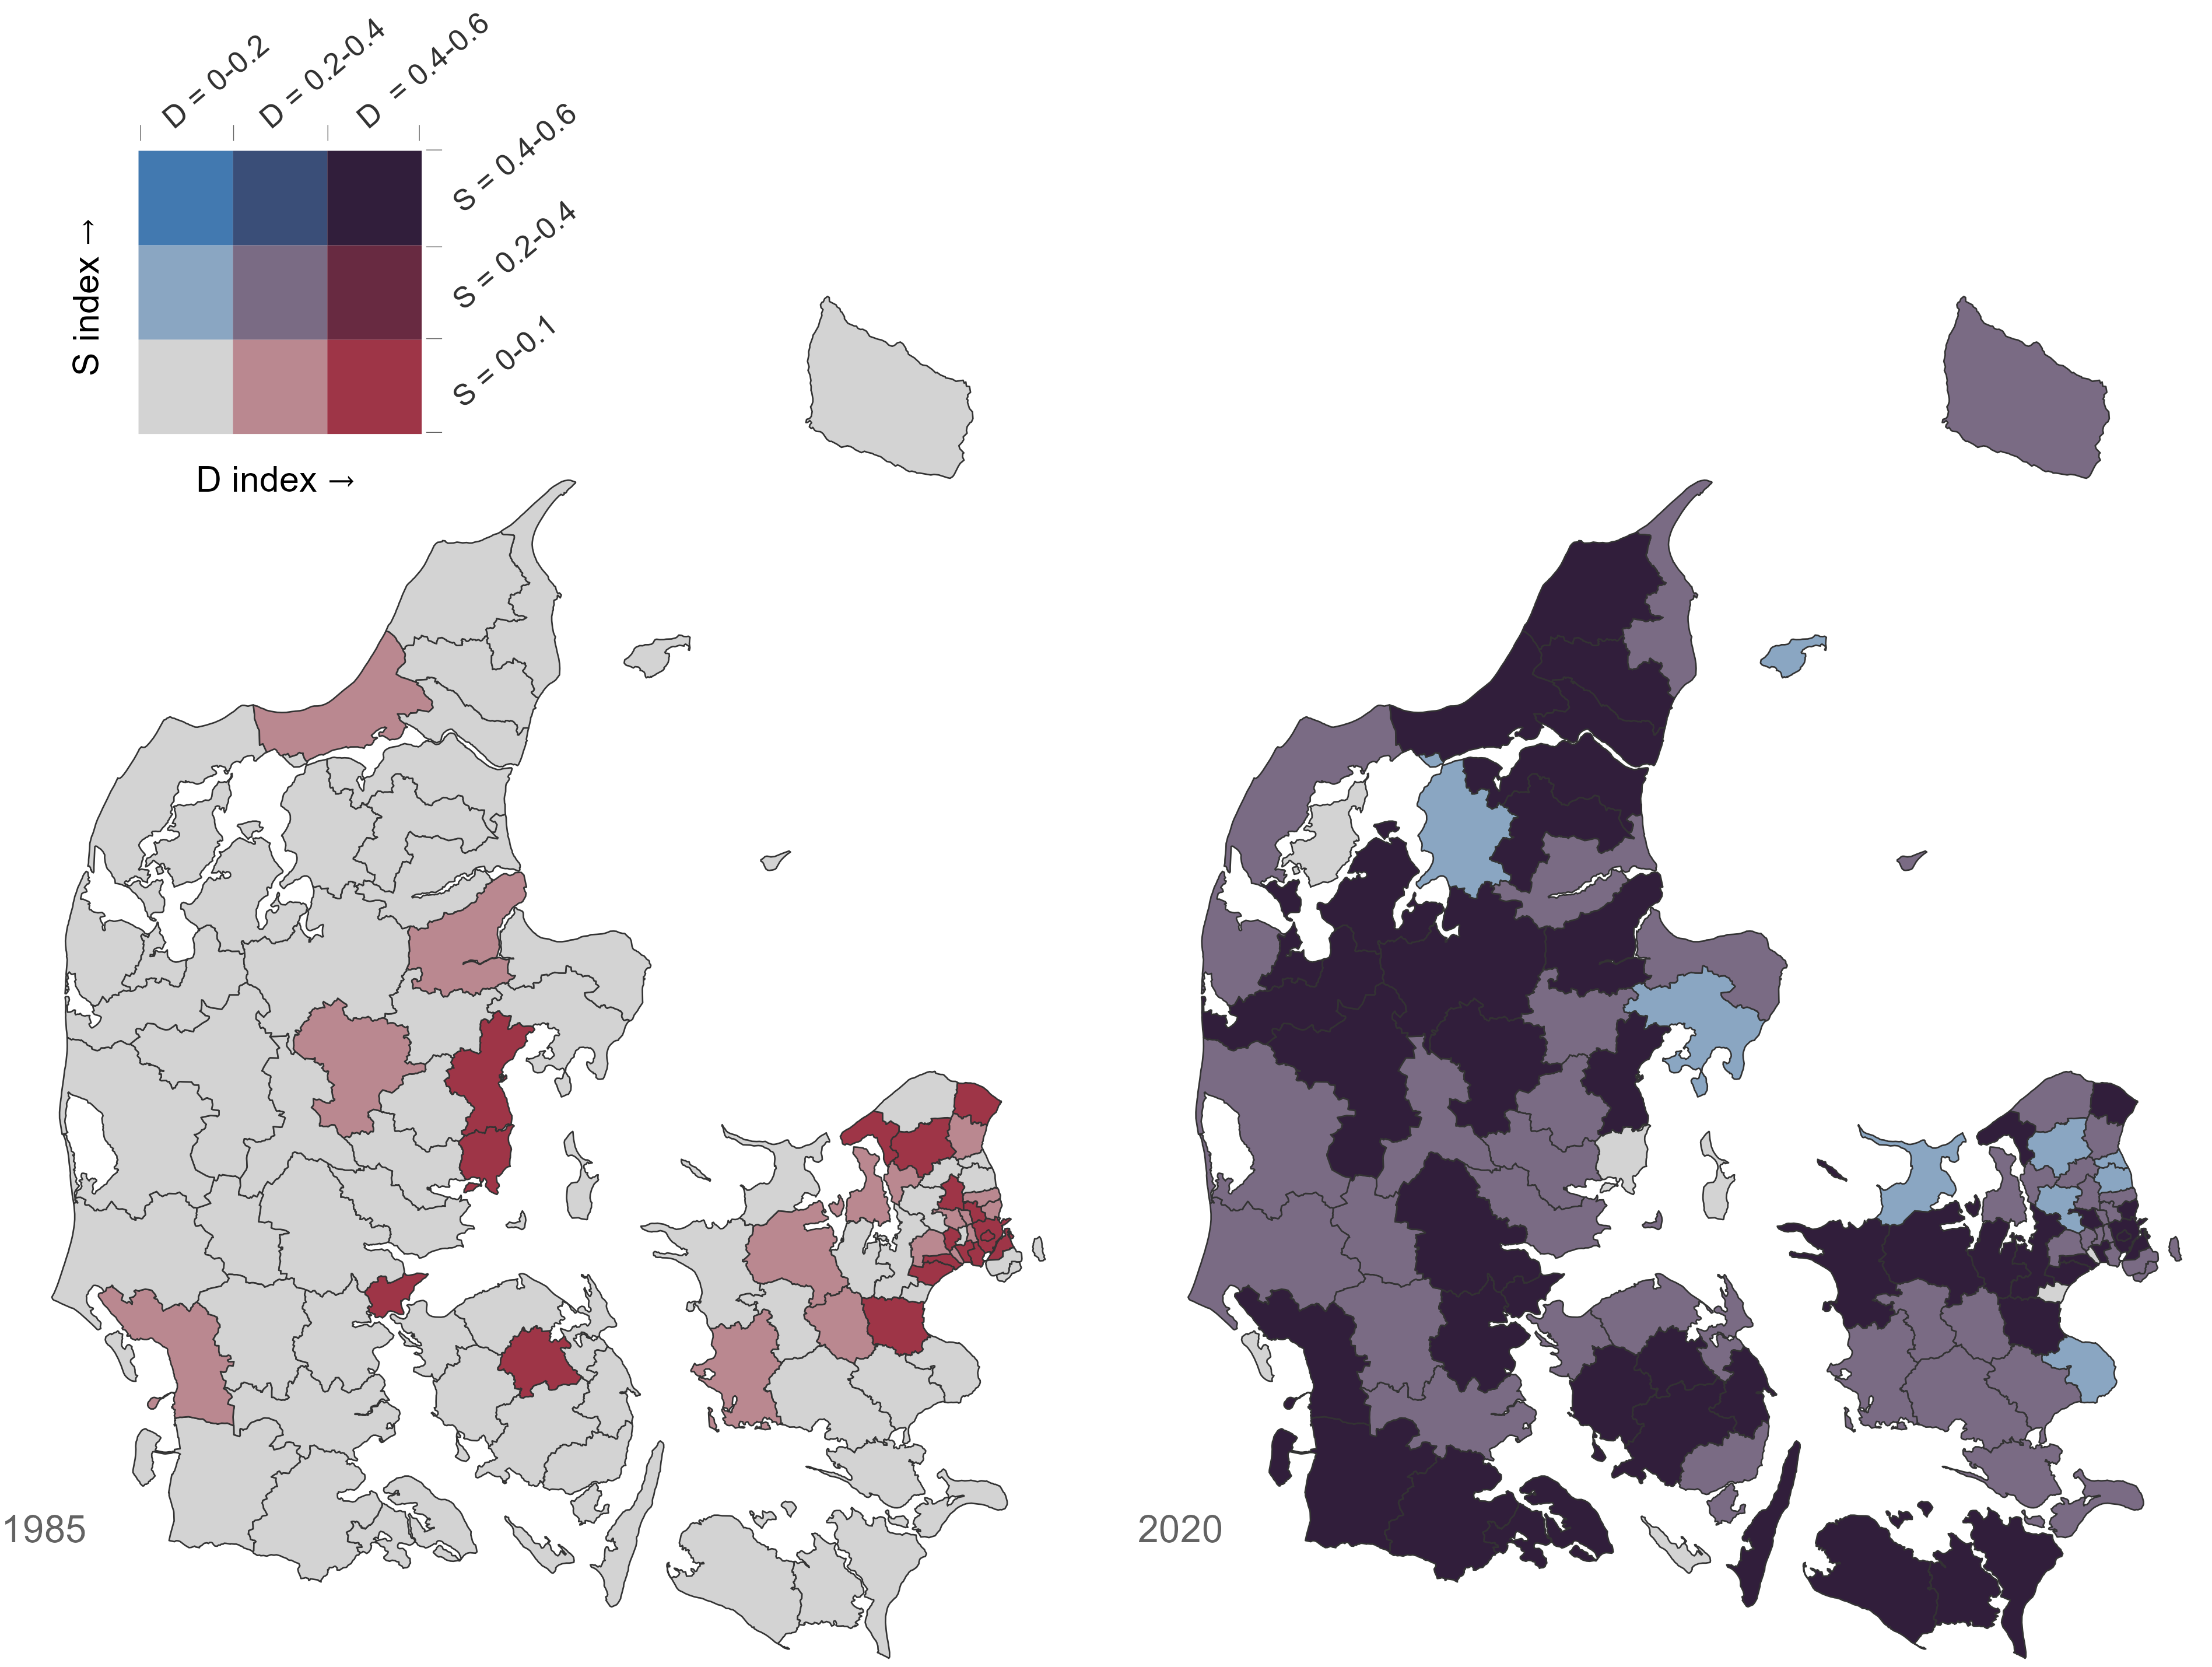
\includegraphics[width=1\linewidth]{images/Figur4} \caption{Etnisk skolesegregering i Danmark på kommunalt niveau, 1985 og 2020}\label{fig:fig-3-3}
\end{figure}

\section{Skolesegregering som produkt af boligsegregering}\label{skolesegregering-som-produkt-af-boligsegregering}

Som det blev diskuteret i \hyperref[det-danske-skolelandskab]{afsnit 1.1}, er der stor variation i koncentrationen af familier med indvandrerbaggrund og afstand mellem skoler. Som andre har vist, er koncentrationen af familier med indvandrerbaggrund ikke kun mellem kommuner, men også inden for kommuner, hvor nogle nabolag er kendetegnet ved høje koncentrationer af minoriteter---i særlig høj grad gældende for den almene boligsektor (\citeproc{ref-andersen2019a}{H. S. Andersen, 2019}; \citeproc{ref-landsbyggefonden2020}{Landsbyggefonden, 2020}). Bemærkelsesværdigt er også, at kommuner med få familier med indvandrerbaggrund angiver, at de ikke ser, at frit skolevalg fører til øget etnisk segregering, mens kommuner med mange familier med indvandrerbaggrund angiver det modsatte (\citeproc{ref-rambuxf8ll2011}{Rambøll, 2011}). Som jeg (\citeproc{ref-larsen2024c}{J. F. Larsen, 2024b}) og andre (\citeproc{ref-boterman2019}{Boterman et al., 2019}; e.g., \citeproc{ref-bunar2010}{Bunar, 2010}; \citeproc{ref-butler2007}{Butler \& Hamnett, 2007}) også har diskuteret, giver det altså en forventning om, at skolesegregering skal forstås i direkte relation til boligsegregering. Fordi de skoler, en familie enten automatisk indskrives i---distriktskolen---eller har mulighed for at vælge som alternativ, helt grundlæggende er betinget af de skoler, der er i nærheden af boligen. Dette indikerer, at mens frit skolevalg har en direkte indflydelse på graden af skolesegregering, er det ikke den primære drivkraft. Boligsegregering, hvor indvandrerfamilier bor koncentreret i bestemte områder og nabolag, spiller en større rolle i at forme de observerede grader af skolesegregering. Denne boligsegregering betyder, at fordi børn med indvandrerbaggrund ofte går i skoler i deres nærområder, hvor der er en højere koncentration af børn med samme baggrund, hvilket bidrager til skolesegregeringen. Kommuner med mange indvandrerfamilier oplever derfor større udfordringer med etnisk skolesegregering, da det frie skolevalg ofte resulterer i, at børn med dansk oprindelse vælger skoler uden for de nærområder med høj koncentration af indvandrerfamilier, hvilket yderligere forstærker segregationen.

Kigger vi på sammenhængen i segregering (\(D\)) på hhv. bolig- og skolemarkedet ser vi i Figur \ref{fig:fig-3-4}, at der er en klar sammenhæng mellem graden af bolig- og skolesegregering i de fleste kommuner, og at denne er stigende over tid (Pearson's \(r=0,50\) i 2020 mod \(r=0,29\) i 1985). Altså, de kommuner med høj boligsegregering har også typisk høj skolesegregering. Skolesegregering kan eksistere med lav boligsegregering---som Rangvid (2007) også diskuterer og viser var aktuelt frem til tidlige 2000'ere i hovedstadsområdet, og som Figur \ref{fig:fig-3-4} også illustrerer for 1985. I de seneste år ser vi en stærk sammenhæng mellem de to typer segregering i de fleste kommuner. Jeg understøtter dette yderligere med en dekomponeringsanalyse i Larsen (\citeproc{ref-larsen2024b}{2024c}). Med andre ord, selvom skolevalget principielt er ubegrænset, er der nogle skoler, der logisk er for langt væk fra hjemmet til, at hverdagen ville kunne hænge sammen. Når familier, der ligner hinanden, bor tættere på andre familier, der ligner dem selv, end de gør med familier, der er forskellige fra dem, vil der være en observerbar tendens til, at børn, som ligner hinanden, også kommer til at gå i skole sammen. Denne tendens er forstærket af at mange forældre vælger skoler baseret på, hvad de opfatter som ``god kvalitet'' og barnets trivsel, kriterier, der ofte er knyttet til skolens omdømme og dets elevgrundlag. Dette fører til, at skoler med mange ressourcestærke elever tiltrækker endnu flere af samme type, mens skoler med mange elever fra mindre ressourcestærke ikke formår at tiltrække nye familier udenfor skoledistriktet. Derfor ser vi, at segregering på boligmarkedet direkte påvirker segregeringen på skolemarkedet, hvilket skaber en selvforstærkende skolesegregerings proces.

\begin{figure}
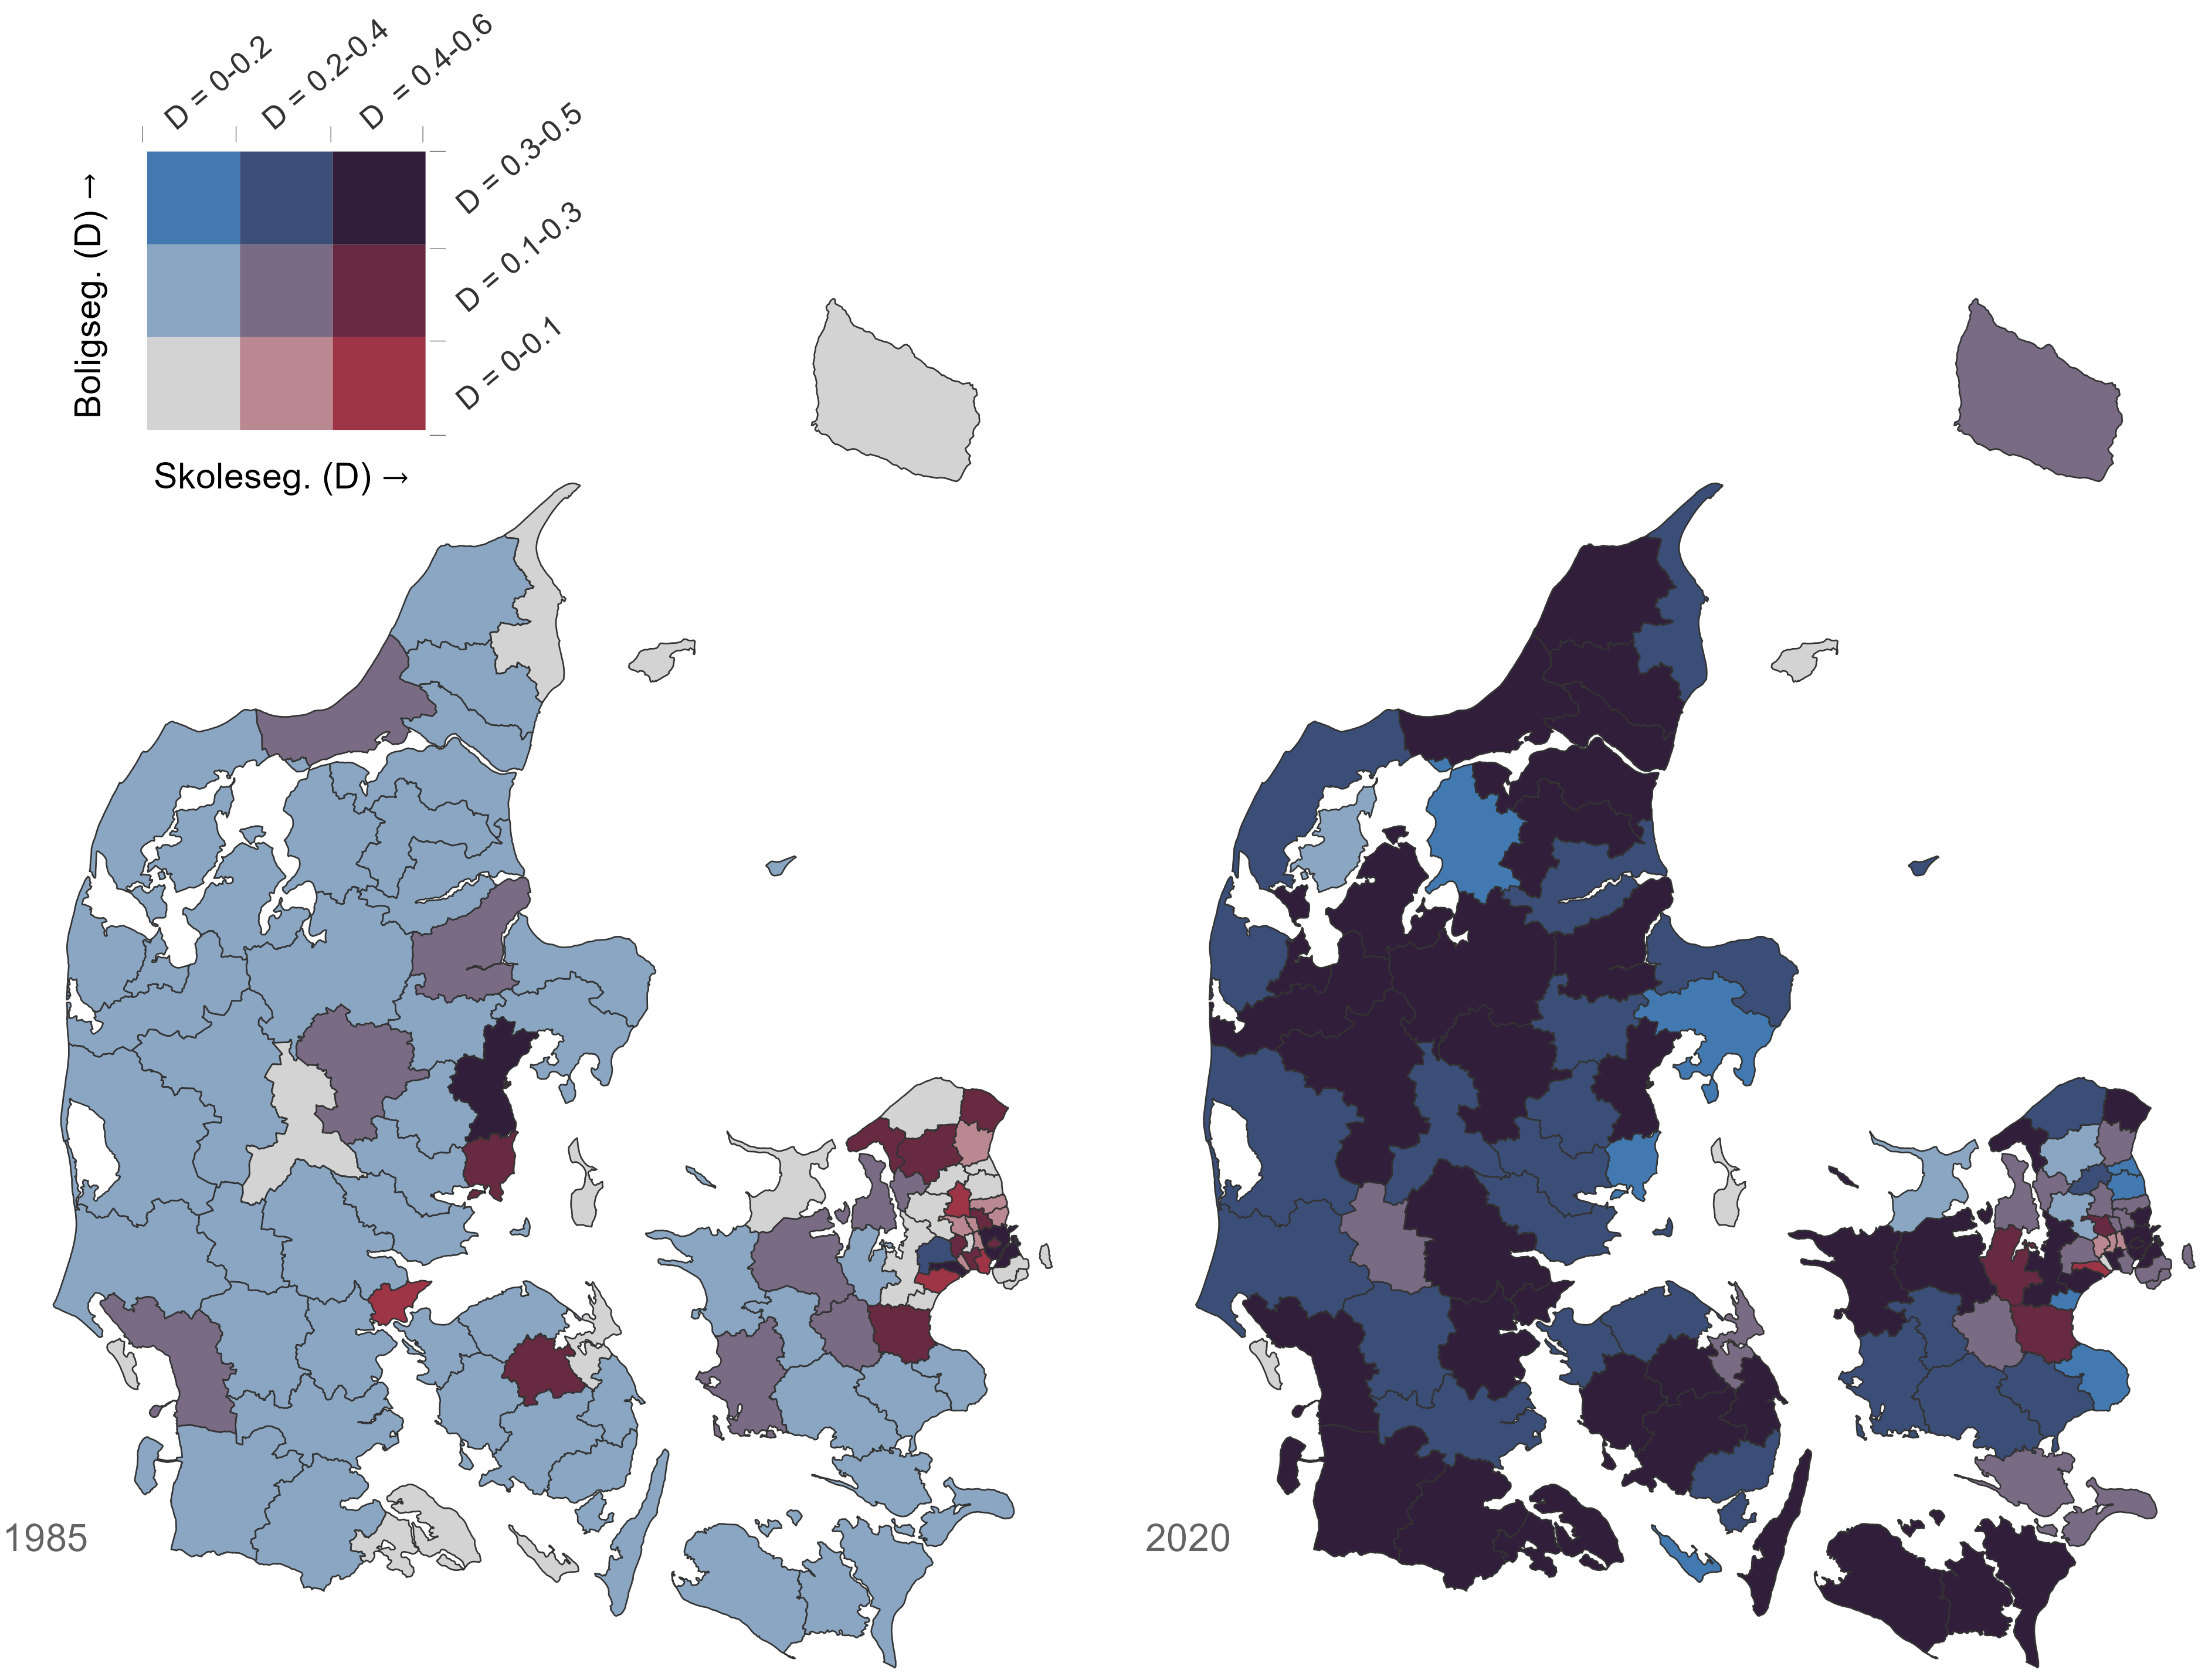
\includegraphics[width=1\linewidth]{images/Figur5} \caption{Etnisk skole- og boligsegregering i Danmark (D indeks) <br> <br> Note: * Boligsegregering er målt blandt personer, der går i den danske grundskole og ikke den fulde population. Boligsegregering er målt på sogneinddelinger og ikke skoledistrikter, da disse kun er tilgængelige for 19 kommuner og årene 2007-2017 i Danmarks Statistiks registre. Måles segregering med afsæt i skoledistrikter er sammenhængen markant mere udpræget (se @larsen2024b).*}\label{fig:fig-3-4}
\end{figure}

\section{Konklusion}\label{konklusion}

Som bidrag til denne bogs undersøgelser og beskrivelser af mødet mellem den etnisk danske befolkning og befolkningen med indvandrerbaggrund i lyset af stigende immigration til Danmark har dette kapitel bidraget med en beskrivelse af, i hvilket omfang den danske grundskole danner et mødested for børn (og deres familier), som ikke ligner hinanden.

Som jeg har beskrevet i dette kapitel, er segregering i det danske grundskolesystem ``kun'' moderat---og segregering har på nogle parametre været faldende over tid på grund af ændrede strukturelle forhold, såsom en større minoritetsbefolkning i de fleste kommuner. Det vil sige, at de danske skoler er mødesteder på tværs af etniske gruppeskel---men omfanget af møder i denne arena er langt fra ``optimalt udnyttet'', og den positive udvikling har været langsom. Samtidig er der tendenser, der tegner et ikke-optimistisk billede af udviklingen. Den langsomme udvikling af mere blandede skoler skal tilskrives den disproportionalt geografiske koncentration af familier med indvandrerbaggrund i bestemte kommuner og nabolag. Dette betyder, at selvom der er potentiale for mere integration i skolerne, begrænses dette i høj grad af, hvor folk bor.

Grunden til at vi interessere os for skolesegregering er selvfølgelig ikke det tekniske oprids af hvorfor segregering kan opstå. Vi er interesseret fordi der er en grundlæggende tro på at det betyder noget for vores samfund, som diskuteret indledningsvist i dette kapitel og i \hyperref[kap1]{kapitel 1}. Børn med dansk oprindelse er blevet mere eksponeret til børn med indvandererbaggrund i en skolekontekst. Fra \(7\%\) i 1985 til \(19\%\) i 2020. Der er altså forventeligt flere sociale relationer på tværs af etniske gruppeskel i de formative år. På den anden side er eksponeringen til andre børn med indvandererbaggrund blandt børn der selv har indvandererbaggrund steget fra \(16\%\) til \(35\%\). Det vil sige at i takt med stigende indvandring og ændrede demografiske forhold i populationen, bliver dele af minoritetsgruppe forholdsvis mere ''isoleret'' i skolelandskabet, grundet en kombination af bosætningsmønstre og tendenser i hvem der udnytter skolevalget.

Så selvom udviklingen ikke er så ekstrem som dele af den offentlige debat anleder til at tro, affejer resultaterne dog ikke en grundlæggende bekymring på lokale niveauer. Mit centrale budskab er, at problemets omfang ikke har rod i eksistensen af frit skolevalg, som andre også argumenterer for (f.eks. Rambøll (\citeproc{ref-rambuxf8ll2011}{2011}) eller Gandil i Zetland (\citeproc{ref-zetland2018}{2018})). Ikke at skolevalget ingen betydning har, men skolevalg øger kun segregering i bestemte områder over det strukturelt bestemte niveau (\citeproc{ref-rangvid2010}{Rangvid, 2010}); skolevalget er ikke den mekanisme, der skaber segregering. I stedet skal skolesegregering forstås først og fremmest som et produkt af bosætningsmønstre, da disse har en fundamental betydning for, hvilke skoler der er tilgængelige for den enkelte familie, uafhængigt af familiens muligheder for at vælge alternativer til distriktskolen. Hvad der yderligere bidrager til skolesegregering er, at disse muligheder samtidig er betinget af, at de alternative skoler rent faktisk har plads til flere elever---hvilket de mest populære skoler sjældent har (\citeproc{ref-rambuxf8ll2011}{Rambøll, 2011}). Dette betyder, at selvom frit skolevalg kan forstærke eksisterende segregeringsmønstre, er det ikke den primære drivkraft bag segregering. For at tackle skolesegregering effektivt, skal vi fokusere på at adressere de underliggende bosætningsmønstre og sikre, at der er tilstrækkelige og attraktive skolemuligheder til rådighed for alle familier, uanset hvor de bor.

\chapter{Arbejdspladser som mødested}\label{kap4}


\includegraphics[width=1\linewidth]{images/dalle-work}

\begin{figure}
\includegraphics[width=1\linewidth]{images/Figur_4_1} \caption{Beskæftigedes med dansk-dansk herkomst gennemsnitlige eksponering til indvandrere/efterkommere på deres arbejdspladsen i 1996 (venstre) og 2019 (højre). <br> <br> **Note**: *Opgjort på tværs af kommuner.*}\label{fig:fig-4-1}
\end{figure}

\begin{figure}
\includegraphics[width=1\linewidth]{images/Figur_4_2} \caption{Andelen af beskæftigede med dansk-dansk herkomst, der ikke er eksponeret til én eneste indvandrer eller efterkommer på deres arbejdsplads i 1996 (venstre) og 2019 (højre). <br> <br> **Note**: *Opgjort på tværs af kommuner. *}\label{fig:fig-4-2}
\end{figure}

\begin{figure}
\includegraphics[width=1\linewidth]{images/Figur_4_3} \caption{Beskæftigedes med dansk-dansk herkomst gennemsnitlige eksponering til MENAPT indvandrere/efterkommer på deres arbejdsplads i 1996 (venstre) og 2019 (højre). <br> <br> **Note**: *Opgjort på tværs af kommuner. MENAPT dækker over ...*}\label{fig:fig-4-3}
\end{figure}

\begin{figure}
\includegraphics[width=1\linewidth]{images/Figur_4_4} \caption{Beskæftigede indvandreres/efterkommeres gennemsnitlige eksponering til beskæftigede med dansk-dansk herkomst på deres arbejdsplads i 1996 (venstre) og 2019 (højre). <br> <br> **Note**: *Opgjort på tværs af kommuner.*}\label{fig:fig-4-4}
\end{figure}

\begin{figure}
\includegraphics[width=1\linewidth]{images/Figur_4_5} \caption{Andelen af beskæftigede indvandrere/efterkommere der ikke er eksponeret til én eneste med dansk-dansk herkomst på deres arbejdsplads i 1996 (venstre) og 2019 (højre). <br> <br> **Note**: *Opgjort på tværs af kommuner.*}\label{fig:fig-4-5}
\end{figure}

\chapter{Foreninger som mødested}\label{kap5}


\includegraphics[width=1\linewidth]{images/dalle-civil}

\chapter{Venskaber -- det første skridt}\label{kap6}


\includegraphics[width=1\linewidth]{images/dalle-friendships}

\chapter{Integration i et kontaktperspektiv}\label{kap7}

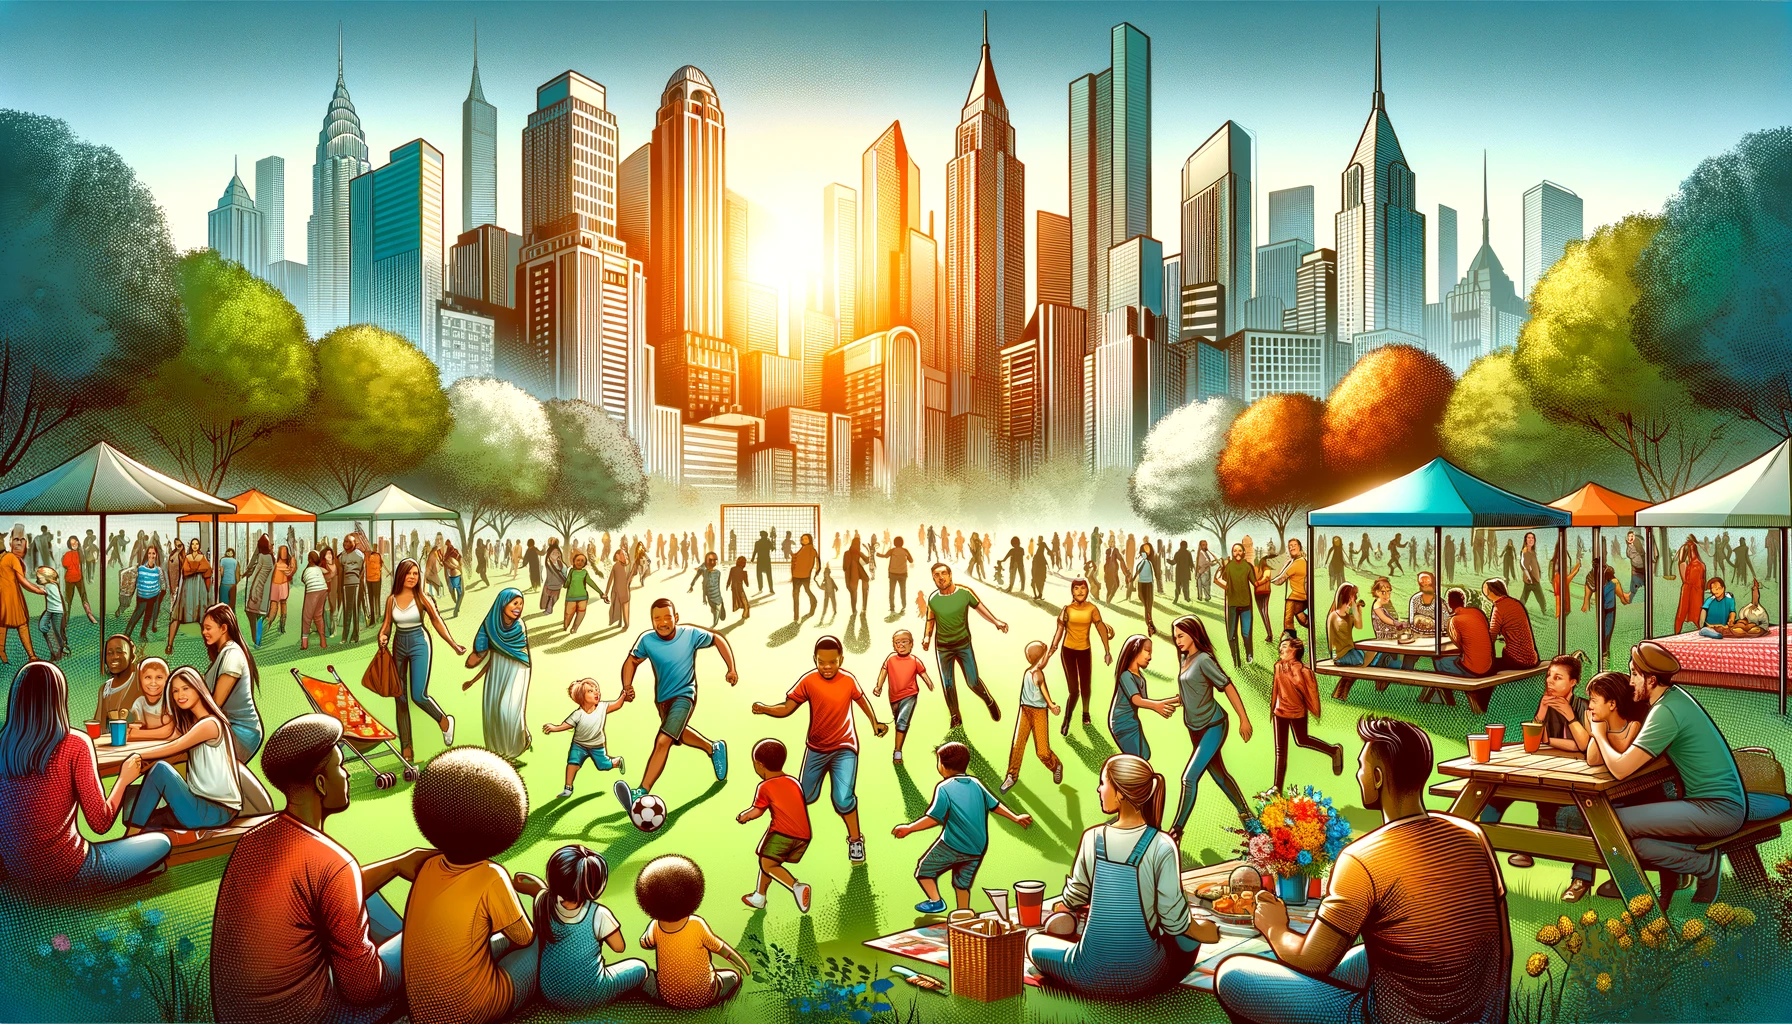
\includegraphics[width=1\linewidth]{images/dalle-integration}

test (\citeproc{ref-xie2015}{Xie, 2015}).

\chapter*{Litteraturliste}\label{litteraturliste}
\addcontentsline{toc}{chapter}{Litteraturliste}

\phantomsection\label{refs}
\begin{CSLReferences}{1}{0}
\bibitem[\citeproctext]{ref-allport1979}
Allport, G. W. (1979). \emph{The nature of prejudice}. Addison-Wesley Pub. Co.

\bibitem[\citeproctext]{ref-andersen2019a}
Andersen, H. S. (2019). \emph{Ethnic spatial segregation in european cities}. Routledge.

\bibitem[\citeproctext]{ref-andersen2019}
Andersen, S. C., \& Guul, T. S. (2019). Reducing minority discrimination at the front line---combined survey and field experimental evidence. \emph{Journal of Public Administration Research and Theory}, \emph{29}(3), 429--444. \url{https://doi.org/10.1093/jopart/muy083}

\bibitem[\citeproctext]{ref-bjerrenielsen2020}
Bjerre-Nielsen, A., \& Gandil, M. H. (2020). \emph{Attendance boundary policies and the limits to combating school segregation}.

\bibitem[\citeproctext]{ref-boterman2019}
Boterman, W., Musterd, S., Pacchi, C., \& Ranci, C. (2019). School segregation in contemporary cities: Socio-spatial dynamics, institutional context and urban outcomes. \emph{Urban Studies}, \emph{56}(15), 3055--3073. \url{https://doi.org/10.1177/0042098019868377}

\bibitem[\citeproctext]{ref-bunar2010}
Bunar, N. (2010). The geographies of education and relationships in a multicultural city: Enrolling in high-poverty, low-performing urban schools and choosing to stay there. \emph{Acta Sociologica}, \emph{53}(2), 141--159. \url{https://doi.org/10.1177/0001699310365732}

\bibitem[\citeproctext]{ref-butler2007}
Butler, T., \& Hamnett, C. (2007). The geography of education: introduction. \emph{Urban Studies}, \emph{44}(7), 1161--1174. \url{https://doi.org/10.1080/00420980701329174}

\bibitem[\citeproctext]{ref-epinion2017}
Epinion. (2017). \emph{Frit skolevalg---hovedrapport}. Undervisningsministeriet.

\bibitem[\citeproctext]{ref-hassan2022}
Hassan, S., Hvidtfeldt, C., Andersen, L. H., \& Udsen, R. O. (2022). Do refugee children impair the academic performance of native children in the school? Informative null results from danish register data. \emph{European Sociological Review}, \emph{39}(3), 352--365. \url{https://doi.org/10.1093/esr/jcac059}

\bibitem[\citeproctext]{ref-hermansen2015}
Hermansen, A. S., \& Birkelund, G. E. (2015). The impact of immigrant classmates on educational outcomes. \emph{Social Forces}, \emph{94}(2), 615--646. \url{https://doi.org/10.1093/sf/sov073}

\bibitem[\citeproctext]{ref-joel2022}
Joel, J. (2002). \emph{Fællesskaberen}. Forlaget Riisvangen.

\bibitem[\citeproctext]{ref-karsten2003}
Karsten, S., Ledoux, G., Roeleveld, J., Felix, C., \& Elshof, D. (2003). School choice and ethnic segregation. \emph{Educational Policy}, \emph{17}(4), 452--477. \url{https://doi.org/10.1177/0895904803254963}

\bibitem[\citeproctext]{ref-kruse2017}
Kruse, H. (2017). \emph{Close neighbors, separate lives}. University of Mannheim.

\bibitem[\citeproctext]{ref-kruse2019}
Kruse, H., \& Kroneberg, C. (2019). More than a sorting machine: Ethnic boundary making in a stratified school system. \emph{American Journal of Sociology}, \emph{125}(2), 431--484.

\bibitem[\citeproctext]{ref-landsbyggefonden2020}
Landsbyggefonden. (2020). \emph{Beboere i den almene boligsektor 2020 - statistik}.

\bibitem[\citeproctext]{ref-larsen2016}
Larsen, C. A. (2016). \emph{Den danske republik: Forandringer i danskernes nationale forestillinger}. Hans Reitzels Forlag.

\bibitem[\citeproctext]{ref-larsen2024a}
Larsen, J. F. (2024a). \emph{Majority and minority exposure in childhood: Studies of ethnic segregation in early life in denmark and its consequences}. Aalborg Universitetsforlag.

\bibitem[\citeproctext]{ref-larsen2024c}
Larsen, J. F. (2024b). Residential mobility among children of native-born danes and children of migrants: Timing, relative risks, and residential sorting. In H. A. G. de Valk (Ed.), \emph{Migrant youth mobility in europe: Patterns, processes and consequences}. Springer.

\bibitem[\citeproctext]{ref-larsen2024b}
Larsen, J. F. (2024c). \emph{Structured school choice: Ethnic school segregation as a byproduct of residential segregation}.

\bibitem[\citeproctext]{ref-leszczensky2015}
Leszczensky, L., \& Pink, S. (2015). Ethnic segregation of friendship networks in school: Testing a rational-choice argument of differences in ethnic homophily between classroom- and grade-level networks. \emph{Social Networks}, \emph{42}, 18--26. \url{https://doi.org/10.1016/j.socnet.2015.02.002}

\bibitem[\citeproctext]{ref-massey1994}
Massey, D. S., \& Denton, N. A. (1994). \emph{American apartheid: Segregation and the making of the underclass}. Harvard University Press.

\bibitem[\citeproctext]{ref-mcpherson2001}
McPherson, M., Smith-Lovin, L., \& Cook, J. M. (2001). Birds of a feather: Homophily in social networks. \emph{Annual Review of Sociology}, \emph{27}(1), 415--444. \url{https://doi.org/10.1146/annurev.soc.27.1.415}

\bibitem[\citeproctext]{ref-nielsen2019}
Nielsen, R. S., \& Andersen, H. T. (2019). Ethnic school segregation in copenhagen: A step in the right direction? \emph{Urban Studies}, \emph{56}(15), 3234--3250. \url{https://doi.org/10.1177/0042098019847625}

\bibitem[\citeproctext]{ref-pettigrew1998}
Pettigrew, T. F. (1998). Reactions toward the new minorities of western europe. \emph{Annual Review of Sociology}, \emph{24}(1), 77--103. \url{https://doi.org/10.1146/annurev.soc.24.1.77}

\bibitem[\citeproctext]{ref-pettigrew2006}
Pettigrew, T. F., \& Tropp, L. R. (2006). A meta-analytic test of intergroup contact theory. \emph{Journal of Personality and Social Psychology}, \emph{90}(5), 751--783. \url{https://doi.org/10.1037/0022-3514.90.5.751}

\bibitem[\citeproctext]{ref-rambuxf8ll2011}
Rambøll. (2011). \emph{Evaluering af mere frit skolevalg (2.0)}.

\bibitem[\citeproctext]{ref-rangvid2010}
Rangvid, B. S. (2010). School choice, universal vouchers and native flight from local schools. \emph{European Sociological Review}, \emph{26}(3), 319--335. \url{https://doi.org/10.1093/esr/jcp024}

\bibitem[\citeproctext]{ref-tropp2005}
Tropp, L. R., \& Pettigrew, T. F. (2005). Relationships between intergroup contact and prejudice among minority and majority status groups. \emph{Psychological Science}, \emph{16}(12), 951--957. \url{https://doi.org/10.1111/j.1467-9280.2005.01643.x}

\bibitem[\citeproctext]{ref-xie2015}
Xie, Y. (2015). \emph{Dynamic documents with {R} and knitr} (2nd ed.). Chapman; Hall/CRC. \url{http://yihui.name/knitr/}

\bibitem[\citeproctext]{ref-zetland2018}
Zetland. (2018). \emph{Fordel danske skolebørn efter en algoritme, siger en forsker. Ellers får vi aldrig lighed i skolerne}. \url{https://www.zetland.dk/historie/soBPENgk-aO9kVR61-0df45}.

\end{CSLReferences}

\appendix


\chapter{Første bilag\ldots{}}\label{bilag1}

This will be Appendix A.

\chapter{Andet bilag\ldots{}}\label{bilag2}

This will be Appendix B.

\end{document}
